\chapter{Biomolécules~: acides aminés, sucres, lipides et nucléotides}\label{ch:b2:biomolecules}

Un édulcorant courant, bien plus sucré que le sucre, est formé de deux acides aminés unis par une seule
liaison amide, l'un d'eux sous forme d'ester méthylique~: l'acide aspartique et la phénylalanine, tous
deux de la configuration qu'utilisent les cellules vivantes. Les molécules du vivant sont construites à
partir de quelques familles de petites unités, acides aminés, sucres, \omterm{def:b2:biomolecules:lipid}{acides gras} et \omterm{def:b2:biomolecules:nucleotide}{nucléotides}, unies
par les réactions des chapitres précédents~: amides, acétals, esters. Ce chapitre les lit comme le fait un
chimiste organicien~: groupes fonctionnels, stéréochimie, comportement acide--base, et réactions qui les
unissent et les coupent.
% ledger: use:aspartame

\begin{recall}
Le volume de première année~: règles CIP, projections de Fischer, chiralité, hémiacétals et acétals,
$\mathrm pK_a$ et diagrammes de distribution, molécules amphiphiles, loi de Biot.
\Cref{ch:b2:acyl-substitution}~: amides, esters, \omterm{def:b2:acyl-substitution:saponification}{saponification}, acides activés. \Cref{ch:b2:amines}~:
les amines comme bases. \Cref{ch:b2:retrosynthesis}~: groupes protecteurs dans une voie de synthèse.
\end{recall}

\section{Acides aminés}

\begin{definition}[Acides aminés]\label{def:b2:biomolecules:amino-acid}
Un \emph{acide $\alpha$-aminé}\index{acide alpha-amine@acide $\alpha$-aminé} \ce{H2N-CHR-COOH} porte un
groupe amino et un groupe acide carboxylique sur le même carbone~; \ce{R} est sa \emph{chaîne
latérale}\index{chaine laterale@chaîne latérale}. Dans l'eau, au voisinage de la neutralité, il existe
sous forme de \emph{zwitterion}\index{zwitterion} (ou amphion),
\ce{H3N+-CHR-COO-}, porteur d'une charge positive et d'une charge négative. Le \emph{point
isoélectrique}\index{point isoelectrique@point isoélectrique} pI est le pH auquel sa charge nette moyenne est nulle.
\end{definition}

Vingt acides aminés construisent les protéines des êtres vivants. Tous sauf la glycine (\ce{R = H}) sont
chiraux, et les acides aminés naturels ont la configuration L (\cref{def:b2:biomolecules:d-l}). Leurs
\omterm{def:b2:biomolecules:amino-acid}{chaînes latérales} les répartissent en familles~: apolaires (alanine, \ce{R = CH3}~; phénylalanine,
\ce{R = CH2C6H5}), polaires, acides (acides aspartique et glutamique, porteurs d'un second groupe
carboxylique) et basiques (lysine, porteuse d'un second groupe amino~; histidine, porteuse d'un cycle imidazole).

\begin{proposition}[Point isoélectrique]\label{prop:b2:biomolecules:pi}
Pour un acide aminé dont la \omterm{def:b2:biomolecules:amino-acid}{chaîne latérale} n'est ni acide ni basique, $\mathrm{pI} = (\mathrm pK_{a1} +
\mathrm pK_{a2})/2$, où $\mathrm pK_{a1}$ est celui du groupe carboxylique et $\mathrm pK_{a2}$ celui du
groupe ammonium. Pour une \omterm{def:b2:biomolecules:amino-acid}{chaîne latérale} acide ou basique, pI est la moyenne des deux $\mathrm pK_a$ qui
encadrent la forme neutre.
\end{proposition}

\begin{proof}
Notons \ce{H2A+} le cation, \ce{HA} le \omterm{def:b2:biomolecules:amino-acid}{zwitterion} et \ce{A-} l'anion. La charge nette est nulle quand
$[\ce{H2A+}] = [\ce{A-}]$. À partir de $K_{a1} = [\ce{HA}]h/[\ce{H2A+}]$ et de $K_{a2} =
[\ce{A-}]h/[\ce{HA}]$, avec $h = [\ce{H3O+}]$, le rapport $[\ce{H2A+}]/[\ce{A-}] = h^2/(K_{a1}K_{a2})$
vaut 1 pour $h^2 = K_{a1}K_{a2}$, c'est-à-dire $\mathrm{pH} = (\mathrm pK_{a1} + \mathrm pK_{a2})/2$. Avec
un troisième groupe ionisable, le même raisonnement s'applique aux deux équilibres qui encadrent la forme
neutre, le troisième groupe étant alors entièrement sous un seul état.
\end{proof}

Pour la glycine, $\mathrm pK_{a1} = 2.35$ et $\mathrm pK_{a2} = 9.78$~: pI $\approx 6.1$. L'acide aspartique
(2.0, 3.9, 9.9) a un pI $\approx 3.0$~; la lysine (2.2, 9.1, 10.7) a un pI $\approx 9.9$.
% ledger: pka:glycine1, pka:glycine2, pka:asp1, pka:asp2, pka:asp3, pka:lys1, pka:lys2, pka:lys3

\begin{omfigure}
\begin{tikzpicture}
\begin{axis}[width=0.47\linewidth, height=5cm, xmin=0, xmax=14, ymin=-2.2, ymax=2.2,
  xlabel={pH}, ylabel={charge nette}, label style={font=\small}, tick label style={font=\scriptsize},
  xtick={0,2,4,6,8,10,12,14}, ytick={-2,-1,0,1,2}, grid=major, grid style={black!12},
  legend style={font=\scriptsize, at={(0.5,1.03)}, anchor=south}, legend columns=3]
\addplot[omDef, thick] table[x=pH, y=gly] {figdata/out/bachelor-2-amino-acid-charge-a.dat};
\addplot[omThm, thick] table[x=pH, y=asp] {figdata/out/bachelor-2-amino-acid-charge-a.dat};
\addplot[omMeth, thick] table[x=pH, y=lys] {figdata/out/bachelor-2-amino-acid-charge-a.dat};
\legend{glycine, acide aspartique, lysine}
\end{axis}
\end{tikzpicture}\hfill
\begin{tikzpicture}
\begin{axis}[width=0.47\linewidth, height=5cm, xmin=0, xmax=14, ymin=0, ymax=1.05,
  xlabel={pH}, ylabel={fraction}, label style={font=\small}, tick label style={font=\scriptsize},
  xtick={0,2,4,6,8,10,12,14},
  legend style={font=\scriptsize, at={(0.5,1.03)}, anchor=south}, legend columns=3]
\addplot[omThm, thick] table[x=pH, y=cation] {figdata/out/bachelor-2-amino-acid-charge-b.dat};
\addplot[omDef, thick] table[x=pH, y=zwitterion] {figdata/out/bachelor-2-amino-acid-charge-b.dat};
\addplot[omMeth, thick] table[x=pH, y=anion] {figdata/out/bachelor-2-amino-acid-charge-b.dat};
\legend{cation, zwitterion, anion}
\end{axis}
\end{tikzpicture}

{\small À gauche~: charge nette de trois acides aminés en fonction du pH, d'après leurs $\mathrm pK_a$ à
\qty{25}{\degreeCelsius}~; chaque courbe coupe zéro au pI. À droite~: les trois formes de la glycine,
\ce{H3N+CH2COOH}, \ce{H3N+CH2COO-} et \ce{H2NCH2COO-}~; le \omterm{def:b2:biomolecules:amino-acid}{zwitterion} prédomine d'environ pH 3 à
pH 9.}
% figdata: bachelor-2/amino-acid-charge.py parts a, b
\end{omfigure}

\begin{method}[Charge nette à un pH donné]\label{met:b2:biomolecules:charge}
\begin{enumerate}
  \item Énumérer tous les groupes ionisables avec leur $\mathrm pK_a$~: le \ce{NH3+} et le \ce{COOH}
        terminaux, et les \omterm{def:b2:biomolecules:amino-acid}{chaînes latérales} ionisables.
  \item Pour chaque groupe, comparer pH et $\mathrm pK_a$~: un groupe est surtout protoné au-dessous de son
        $\mathrm pK_a$, surtout déprotoné au-dessus (à plus d'une unité~: à plus de 90~\%).
  \item Additionner les charges~: \ce{NH3+} $+1$, \ce{NH2} 0, \ce{COOH} 0, \ce{COO-} $-1$ (imidazolium $+1$).
  \item Près d'un $\mathrm pK_a$, compter ce groupe comme à moitié chargé~; pour une valeur exacte, utiliser les fractions
        $1/(1 + 10^{\mathrm pK_a - \mathrm{pH}})$.
\end{enumerate}
\end{method}

\section{Peptides}

\begin{definition}[Peptides]\label{def:b2:biomolecules:peptide}
La liaison amide formée entre le groupe carboxylique d'un acide aminé et le groupe amino d'un autre est
une \emph{liaison peptidique}\index{liaison peptidique}~; une chaîne d'acides aminés unis par des
liaisons peptidiques est un \emph{peptide}\index{peptide} (une protéine quand elle est longue), qu'on
écrit de son extrémité amino libre (N-terminale) à son extrémité carboxylique libre (C-terminale). Un
\emph{couplage peptidique}\index{couplage peptidique} forme une liaison peptidique au laboratoire au
moyen d'un \emph{agent de couplage}\index{agent de couplage}, réactif qui transforme le groupe
carboxylique en un dérivé activé dans des conditions douces (un carbodiimide, par exemple).
\end{definition}

\begin{omfigure}
\setchemfig{atom sep=1.9em}
\schemestart
\chemfig{R-C(=[2]O)-N(-[6]H)-R'}
\arrow{<->}
\chemfig{R-C(-[2]\chemabove{O}{\scriptstyle -})=\chemabove{N}{\scriptstyle +}(-[6]H)-R'}
\schemestop
\par\vspace{6pt}

{\small Les deux formes mésomères de la \omterm{def:b2:biomolecules:peptide}{liaison peptidique}. Le doublet de l'azote est partagé avec le
carbonyle~: la liaison \ce{C-N} a un caractère partiel de double liaison, et les six atomes C, C, O, N,
H, C sont dans un même plan.}
\end{omfigure}

\begin{proposition}[Une liaison plane]\label{prop:b2:biomolecules:planar}
La \omterm{def:b2:biomolecules:peptide}{liaison peptidique} est plane, la rotation autour de la liaison \ce{C-N} est bloquée, et l'azote de
l'amide n'est ni basique ni nucléophile.
\end{proposition}

\begin{proof}[Argument]
La seconde forme mésomère donne à la liaison \ce{C-N} une part de caractère de double liaison~: la faire
tourner romprait le recouvrement du doublet de l'azote avec le système $\pi$ de \ce{C=O}, ce qui coûte de
l'énergie, si bien que les atomes qui l'entourent restent dans un même plan, la disposition trans (les
deux carbones de la chaîne de part et d'autre de la liaison \ce{C-N}) étant la disposition habituelle.
Le doublet engagé dans la résonance n'est pas disponible pour un proton ou un électrophile, comme pour
tout amide (\cref{ch:b2:acyl-substitution}). Les protéines se replient autour de chaînes de ces plans rigides.
\end{proof}

\begin{proposition}[Pourquoi protéger et activer]\label{prop:b2:biomolecules:coupling}
Préparer un dipeptide donné à partir de deux acides aminés exige à la fois la protection des groupes qui
ne doivent pas réagir et l'activation du groupe carboxylique qui doit réagir.
\end{proposition}

\begin{proof}[Argument]
Un acide carboxylique et une amine mélangés à température ambiante donnent un sel, et non un amide~;
chauffer pour chasser l'eau racémiserait en outre les acides aminés. Une activation (\omterm{def:b2:acyl-substitution:derivative}{chlorure d'acyle},
anhydride ou \omterm{def:b2:biomolecules:peptide}{agent de couplage}) est donc nécessaire. Mais chaque acide aminé porte les deux groupes~:
activer un mélange de glycine et d'alanine donnerait Gly--Ala, Ala--Gly, Gly--Gly, Ala--Ala et des
chaînes plus longues. Bloquer l'amine du premier et l'acide du second ne laisse qu'une seule liaison possible.
\end{proof}

\begin{method}[Synthèse d'un dipeptide]\label{met:b2:biomolecules:peptide}
\begin{enumerate}
  \item Protéger le groupe amino de l'acide aminé N-terminal (sous forme de carbamate, par exemple un
        groupe \textit{tert}-butoxycarbonyle).
  \item Protéger le groupe carboxylique de l'acide aminé C-terminal (sous forme d'ester méthylique ou
        benzylique), ainsi que toute \omterm{def:b2:biomolecules:amino-acid}{chaîne latérale} réactive.
  \item Activer le groupe carboxylique libre par un \omterm{def:b2:biomolecules:peptide}{agent de couplage} et ajouter le partenaire protégé~:
        une \omterm{def:b2:biomolecules:peptide}{liaison peptidique} se forme.
  \item Retirer les groupes protecteurs, de préférence un jeu orthogonal
        (\cref{def:b2:retrosynthesis:orthogonal})~; pour continuer, ne retirer que la protection de
        l'amine et recommencer.
\end{enumerate}
\end{method}

Répéter le cycle de nombreuses fois en solution exigerait une purification à chaque étape. Dans la
synthèse sur support solide, la chaîne en croissance est fixée par son extrémité C-terminale à une bille
de \omterm{def:b2:polymer-synthesis:polymer}{polymère}~; les réactifs en excès et les sous-produits sont éliminés par lavage après chaque couplage,
et le \omterm{def:b2:biomolecules:peptide}{peptide} achevé est détaché du support à la fin.

\begin{omfigure}
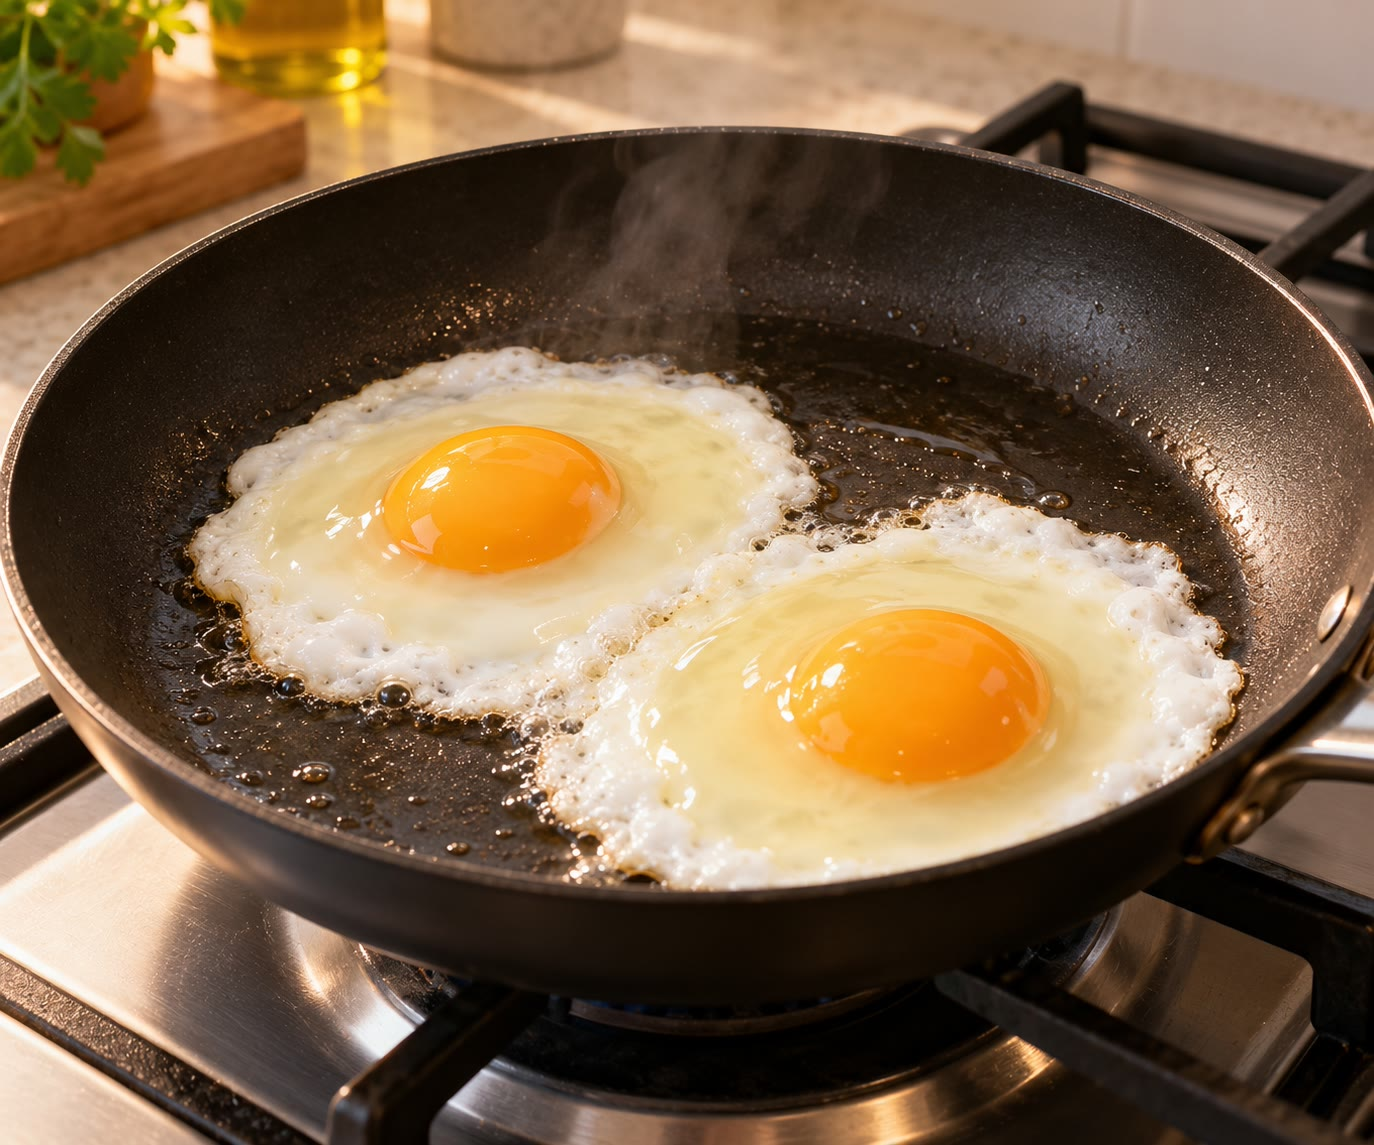
\includegraphics[width=0.5\linewidth]{images/book3/ai/b2-30-eggs.jpg}

{\small Œufs au plat en train de cuire. Les protéines du blanc se déplient à la chaleur et se lient les
unes aux autres~: le liquide translucide devient un solide blanc opaque. Aucune \omterm{def:b2:biomolecules:peptide}{liaison peptidique} n'est
rompue~; le changement porte sur la façon dont les chaînes sont repliées (illustration).}
\end{omfigure}

\section{Glucides}

\begin{definition}[D et L]\label{def:b2:biomolecules:d-l}
Un sucre ou un acide aminé est dessiné en projection de Fischer avec son carbone le plus oxydé en haut.
Il est D si le \ce{OH} du stéréocentre le plus éloigné du haut (ou, pour un acide $\alpha$-aminé, le
\ce{NH2} du carbone $\alpha$) pointe vers la droite, et L s'il pointe vers la gauche. Ces descripteurs
comparent les configurations à celle du glycéraldéhyde~; ce ne sont pas les descripteurs CIP.
\end{definition}

\begin{definition}[Oses]\label{def:b2:biomolecules:sugar}
Un \emph{ose}\index{ose} (ou monosaccharide) est un aldéhyde ou une cétone polyhydroxylé, en général
\ce{C_nH_{2n}O_n} avec $n$ de 3 à 7, qui ne peut pas être hydrolysé en sucres plus petits. Un
\emph{aldose}\index{aldose} porte un groupe aldéhyde en C1, un \emph{cétose}\index{cetose@cétose} un
groupe cétone, en général en C2. Le glucose est un aldohexose, le fructose un cétohexose.
\end{definition}

Dans l'eau, un aldohexose est presque entièrement cyclique~: le \ce{OH} de C5 s'additionne sur
l'aldéhyde, en formant un cycle hémiacétal à six atomes (un pyranose). La cyclisation crée un nouveau
stéréocentre en C1.

\begin{definition}[Anomères]\label{def:b2:biomolecules:anomer}
Dans une \emph{projection de Haworth}\index{projection de Haworth}, le cycle d'un sucre cyclique est
dessiné à plat, perpendiculaire à la page, avec son oxygène à l'arrière à droite et ses substituants
au-dessus ou au-dessous du cycle. Le carbone de l'hémiacétal (C1 d'un \omterm{def:b2:biomolecules:sugar}{aldose}) est le \emph{carbone
anomère}\index{carbone anomere@carbone anomère}~; les deux configurations qu'il peut prendre donnent deux
diastéréoisomères, les \emph{anomères}\index{anomeres@anomères}~: pour un sucre D, l'anomère $\alpha$ a le
\ce{OH} anomère au-dessous du cycle (à l'opposé du \ce{CH2OH}), l'anomère $\beta$ au-dessus. Dans l'eau,
les anomères s'interconvertissent en passant par la chaîne ouverte, et le pouvoir rotatoire d'un anomère
fraîchement dissous dérive vers une valeur d'équilibre~: c'est la \emph{mutarotation}\index{mutarotation}.
\end{definition}

\begin{omfigure}
\setchemfig{atom sep=1.7em}
\begin{minipage}[c]{0.24\linewidth}\centering
\chemfig{CHO-[6]C(-[4]H)(-[0]OH)-[6]C(-[4,,,2]HO)(-[0]H)-[6]C(-[4]H)(-[0]OH)-[6]C(-[4]H)(-[0]OH)-[6]CH_2OH}
\end{minipage}%
\begin{minipage}[c]{0.37\linewidth}\centering
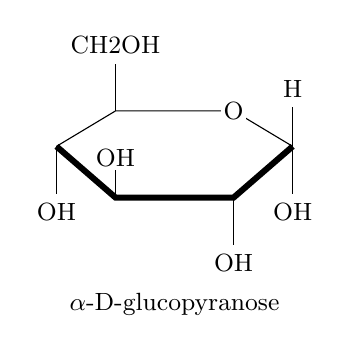
\begin{tikzpicture}[x=1cm, y=1cm, font=\small]
\coordinate (C4) at (-1.5,0); \coordinate (C3) at (-0.75,-0.65); \coordinate (C2) at (0.75,-0.65);
\coordinate (C1) at (1.5,0); \coordinate (O) at (0.75,0.45); \coordinate (C5) at (-0.75,0.45);
\draw (C5) -- (O) -- (C1); \draw (C4) -- (C5);
\draw[line width=2.2pt] (C4) -- (C3) -- (C2) -- (C1);
\node[fill=white, inner sep=1pt] at (O) {O};
\draw (C5) -- ++(0,0.6) node[above] {\ce{CH2OH}};
\draw (C1) -- ++(0,-0.6) node[below] {OH}; \draw (C1) -- ++(0,0.5) node[above] {H};
\draw (C2) -- ++(0,-0.6) node[below] {OH}; \draw (C3) -- ++(0,0.35) node[above, inner sep=1pt] {OH};
\draw (C4) -- ++(0,-0.6) node[below] {OH};
\node at (0,-2.0) {$\alpha$-D-glucopyranose};
\end{tikzpicture}
\end{minipage}%
\begin{minipage}[c]{0.37\linewidth}\centering
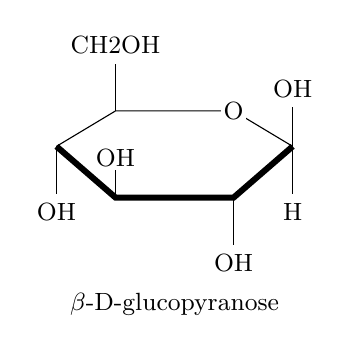
\begin{tikzpicture}[x=1cm, y=1cm, font=\small]
\coordinate (C4) at (-1.5,0); \coordinate (C3) at (-0.75,-0.65); \coordinate (C2) at (0.75,-0.65);
\coordinate (C1) at (1.5,0); \coordinate (O) at (0.75,0.45); \coordinate (C5) at (-0.75,0.45);
\draw (C5) -- (O) -- (C1); \draw (C4) -- (C5);
\draw[line width=2.2pt] (C4) -- (C3) -- (C2) -- (C1);
\node[fill=white, inner sep=1pt] at (O) {O};
\draw (C5) -- ++(0,0.6) node[above] {\ce{CH2OH}};
\draw (C1) -- ++(0,0.5) node[above] {OH}; \draw (C1) -- ++(0,-0.6) node[below] {H};
\draw (C2) -- ++(0,-0.6) node[below] {OH}; \draw (C3) -- ++(0,0.35) node[above, inner sep=1pt] {OH};
\draw (C4) -- ++(0,-0.6) node[below] {OH};
\node at (0,-2.0) {$\beta$-D-glucopyranose};
\end{tikzpicture}
\end{minipage}
\par\vspace{6pt}

{\small Le D-glucose. À gauche~: la chaîne ouverte en projection de Fischer, \ce{OH} de C5 à droite (D).
Au milieu et à droite~: les deux \omterm{def:b2:biomolecules:anomer}{anomères} pyranose en \omterm{def:b2:biomolecules:anomer}{projection de Haworth}~; les groupes situés à droite
dans la projection de Fischer pointent vers le bas, ceux de gauche vers le haut, et C5 porte le \ce{CH2OH}
vers le haut. Les \omterm{def:b2:biomolecules:anomer}{anomères} ne diffèrent qu'en C1. Les hydrogènes de C2 à C5 sont omis.}
\end{omfigure}

\begin{method}[De Fischer à Haworth (D-aldopyranose)]\label{met:b2:biomolecules:haworth}
\begin{enumerate}
  \item Dessiner le cycle avec O à l'arrière à droite, C1 à droite, puis C2, C3, C4 dans le sens horaire
        le long de l'avant et de la gauche, C5 à l'arrière à gauche.
  \item Les groupes situés à droite dans la projection de Fischer vont vers le bas, ceux de gauche vers le haut.
  \item Sur C5 (série D), le \ce{CH2OH} va vers le haut.
  \item Sur C1, le \ce{OH} va vers le bas pour $\alpha$, vers le haut pour $\beta$.
\end{enumerate}
\end{method}

\begin{proposition}[Équilibre de mutarotation]\label{prop:b2:biomolecules:mutarotation}
Si les pouvoirs rotatoires spécifiques des \omterm{def:b2:biomolecules:anomer}{anomères} purs valent $[\alpha]_\alpha$ et $[\alpha]_\beta$ et
celui du mélange à l'équilibre $[\alpha]_{\mathrm{eq}}$, la fraction molaire de l'anomère $\alpha$ à
l'équilibre vaut
\begin{equation*}
x_\alpha = \frac{[\alpha]_{\mathrm{eq}} - [\alpha]_\beta}{[\alpha]_\alpha - [\alpha]_\beta}.
\end{equation*}
\end{proposition}

\begin{proof}
La chaîne ouverte représente une infime fraction du mélange et est négligée. Les pouvoirs rotatoires des
deux \omterm{def:b2:biomolecules:anomer}{anomères} s'additionnent en proportion de leurs concentrations (loi de Biot, volume de première
année)~; comme ils ont la même masse molaire, $[\alpha]_{\mathrm{eq}} = x_\alpha[\alpha]_\alpha + (1 - x_\alpha)[\alpha]_\beta$,
équation que l'on résout pour $x_\alpha$.
\end{proof}

Le D-glucose à l'équilibre dans l'eau a $[\alpha] = +52.7$ (en \unit{\degree\,dm^{-1}\,g^{-1}\,mL}).
Avec des pouvoirs rotatoires des \omterm{def:b2:biomolecules:anomer}{anomères} de $+112$ et $+18.7$ (données de l'exercice), $x_\alpha = (52.7 - 18.7)/(112 - 18.7)
\approx 0.36$~: environ 36~\% d'$\alpha$ et 64~\% de $\beta$. L'anomère $\beta$, dont tous les
substituants sont équatoriaux dans la chaise, est le plus stable.
% ledger: rot:glucose-eq

\begin{definition}[Glycosides]\label{def:b2:biomolecules:glycoside}
Un \emph{glycoside}\index{glycoside} est l'acétal formé quand le \ce{OH} anomère d'un sucre est remplacé
par un groupe \ce{OR} issu d'un alcool, souvent un autre sucre~; la liaison entre le \omterm{def:b2:biomolecules:anomer}{carbone anomère} et
cet oxygène est la \emph{liaison glycosidique}\index{liaison glycosidique}. Un \emph{sucre
réducteur}\index{sucre reducteur@sucre réducteur} est un sucre qui réduit des oxydants doux comme la
liqueur de Fehling ou le réactif de Tollens.
\end{definition}

\begin{proposition}[Réducteur ou non]\label{prop:b2:biomolecules:reducing}
Un sucre porteur d'un groupe hémiacétal (ou hémicétal) libre est réducteur~; un \omterm{def:b2:biomolecules:glycoside}{glycoside} dont tous les
\omterm{def:b2:biomolecules:anomer}{carbones anomères} sont engagés dans des \omterm{def:b2:biomolecules:glycoside}{liaisons glycosidiques} ne l'est pas.
\end{proposition}

\begin{proof}[Argument]
Un hémiacétal est en équilibre avec la chaîne ouverte, dont le groupe aldéhyde est oxydé par le
réactif~; l'équilibre ouvre alors de nouveaux cycles jusqu'à ce que tout le sucre ait réagi. Un acétal ne
s'ouvre pas dans l'eau neutre ou basique~: le \omterm{def:b2:biomolecules:anomer}{carbone anomère} reste bloqué, sans aldéhyde à oxyder.
\end{proof}

Le maltose (deux glucoses, C1 de l'un lié à O4 de l'autre) conserve un hémiacétal libre et est
réducteur~; le saccharose relie l'un à l'autre les \omterm{def:b2:biomolecules:anomer}{carbones anomères} du glucose et du fructose et ne
l'est pas. L'amidon et la cellulose sont tous deux des chaînes de glucose unies C1--O4~: $\alpha$ dans
l'amidon, qui s'enroule et se digère~; $\beta$ dans la cellulose, dont les chaînes droites s'empilent en
fibres maintenues par des liaisons hydrogène.

\section{Lipides}

\begin{definition}[Lipides]\label{def:b2:biomolecules:lipid}
Un \emph{acide gras}\index{acide gras} est un acide carboxylique à longue chaîne non ramifiée, en
général de 12 à 22 carbones, saturée ou porteuse de doubles liaisons (\textit{Z}). Un
\emph{triglycéride}\index{triglyceride@triglycéride} est le triester du propane-1,2,3-triol (glycérol)
et de trois acides gras. Un \emph{phospholipide}\index{phospholipide} est un diester du glycérol et de
deux acides gras dont la troisième position porte un groupe phosphate lié à un petit groupe polaire.
\end{definition}

Les doubles liaisons (\textit{Z}) coudent les chaînes, qui s'empilent alors mal~: l'acide stéarique
(18 carbones, saturé) fond à \qty{69}{\degreeCelsius}, l'acide oléique (18 carbones, une double liaison
\textit{Z}) à \qty{13}{\degreeCelsius}. Les graisses riches en chaînes saturées sont solides à
température ambiante~; les huiles, riches en chaînes insaturées, sont liquides. Les \omterm{def:b2:biomolecules:lipid}{triglycérides} se
saponifient en glycérol et en savons (\cref{ch:b2:acyl-substitution}).
% ledger: mp:stearic, mp:oleic

\begin{omfigure}
\begin{tikzpicture}[x=1cm, y=1cm]
\foreach \i in {0,1,2,3,4,5,6,7,8,9}{
  \fill[omDef!60] (0.6*\i,1.6) circle (0.17);
  \draw[thick, black!70] (0.6*\i-0.06,1.43) .. controls (0.6*\i-0.12,1.2) and (0.6*\i,1.0) .. (0.6*\i-0.06,0.75);
  \draw[thick, black!70] (0.6*\i+0.06,1.43) .. controls (0.6*\i+0.12,1.2) and (0.6*\i,1.0) .. (0.6*\i+0.06,0.75);
  \fill[omDef!60] (0.6*\i,-0.6) circle (0.17);
  \draw[thick, black!70] (0.6*\i-0.06,-0.43) .. controls (0.6*\i-0.12,-0.2) and (0.6*\i,0.0) .. (0.6*\i-0.06,0.25);
  \draw[thick, black!70] (0.6*\i+0.06,-0.43) .. controls (0.6*\i+0.12,-0.2) and (0.6*\i,0.0) .. (0.6*\i+0.06,0.25);
}
\node[font=\small, anchor=west] at (6.0,2.2) {eau};
\node[font=\small, anchor=west] at (6.0,0.5) {cœur hydrocarboné};
\node[font=\small, anchor=west] at (6.0,-1.2) {eau};
\draw[densely dotted] (5.6,1.6) -- (6.0,1.6) node[right, font=\footnotesize] {têtes polaires};
\draw[densely dotted] (5.6,1.05) -- (6.0,1.05) node[right, font=\footnotesize] {deux queues d'acide gras};
\end{tikzpicture}
\par\vspace{4pt}

{\small Une bicouche de \omterm{def:b2:biomolecules:lipid}{phospholipides}, schématique~: les têtes polaires font face à l'eau des deux
côtés, les queues hydrocarbonées se rejoignent à l'intérieur. Les membranes cellulaires reposent sur
cette structure~; les savons, qui n'ont qu'une queue par tête, forment plutôt de petites sphères dont
les queues sont à l'intérieur, appelées micelles.}
\end{omfigure}

\section{Nucléotides}

\begin{definition}[Nucléotides]\label{def:b2:biomolecules:nucleotide}
Une \emph{base nucléique}\index{base nucleique@base nucléique} est un hétérocycle azoté~: l'adénine (A) et
la guanine (G), des purines~; la cytosine (C), la thymine (T) et l'uracile (U), des pyrimidines. Un
\emph{nucléoside}\index{nucleoside@nucléoside} est une base nucléique liée par un azote au C1 du ribose
ou du 2-désoxyribose (un $N$-glycoside). Un \emph{nucléotide}\index{nucleotide@nucléotide} est un ester
phosphorique d'un nucléoside. Dans les acides nucléiques, les nucléotides sont unis par des \emph{liaisons
phosphodiester}\index{liaison phosphodiester}~: un phosphate relie O3 d'un sucre à O5 du suivant.
\end{definition}

L'ADN utilise le 2-désoxyribose et les bases A, G, C, T~; l'ARN utilise le ribose et U à la place de T. La
chaîne a un sens, de son extrémité 5$'$ à son extrémité 3$'$, et les phosphates, ionisés au pH
physiologique, en font un polyanion. Deux brins d'ADN sont orientés en sens opposés et maintenus
ensemble par des liaisons hydrogène entre bases se faisant face.

\begin{proposition}[Appariement des bases]\label{prop:b2:biomolecules:pairing}
Dans l'ADN double brin, l'adénine s'apparie à la thymine par deux liaisons hydrogène, et la guanine à la
cytosine par trois.
\end{proposition}

\begin{proof}[Argument]
Les paires sont celles dont les bords font correspondre des donneurs (\ce{N-H}) et des accepteurs
(oxygène de \ce{C=O}, azote du cycle) aux bonnes distances, une purine faisant face à une pyrimidine pour
que toutes les paires aient la même largeur. A offre \ce{N-H} (son groupe amino) et un \ce{N} du cycle~;
T offre \ce{C=O} et \ce{N-H}~: deux liaisons. G offre \ce{C=O}, \ce{N-H} et \ce{N-H} (amino)~; C offre
\ce{N-H} (amino), \ce{N} et \ce{C=O}~: trois liaisons. La figure les montre.
\end{proof}

\begin{omfigure}
\setchemfig{atom sep=1.7em}
\chemfig{?[a](-[:90]CH_3)-[:-30](=[:30]@{to}O)-[:-90]N(-[:-30]@{th}H)-[:-150](=[:-90]O)-[:150]N(-[:-150]R)-[:90]?[a,2]}%
\hspace{2.3em}%
\raisebox{-1.0em}{\chemfig{?[a](-[:150]N(-[:90]H)-[:210]@{ah}H)-[:30]?[b](-[:78]N=[:6]-[:-66]N(-[:-30]R)-[:-138]?[c])=[:-30]?[c]-[:-90]N=[:-150]-[:150]@{an}N?[a,2]}}
\chemmove{\draw[-, densely dotted, thick](to)--(ah); \draw[-, densely dotted, thick](th)--(an);}
\hspace{1.5em}
\chemfig{?[a]-[:-30](-[:30]N(-[:90]H)-[:-30]@{ch}H)=[:-90]@{cn}N-[:-150](=[:-90]@{co}O)-[:150]N(-[:-150]R)-[:90]?[a,2]}%
\hspace{2.3em}%
\raisebox{-0.6em}{\chemfig{?[a](=[:150]@{go}O)-[:30]?[b](-[:78]N=[:6]-[:-66]N(-[:-30]R)-[:-138]?[c])=[:-30]?[c]-[:-90]N=[:-150](-[:-90]N(-[:-30]H)-[:-150]@{gh}H)-[:150]N?[a](-[:180]@{gn}H)}}
\chemmove{\draw[-, densely dotted, thick](ch)--(go); \draw[-, densely dotted, thick](cn)--(gn);
  \draw[-, densely dotted, thick](co)--(gh);}
\par\vspace{6pt}

{\small Les deux paires de bases de l'ADN. À gauche~: thymine et adénine, deux liaisons hydrogène (en
pointillés). À droite~: cytosine et guanine, trois. R est le désoxyribose de chaque brin~; les deux
groupes R d'une paire pointent du même côté, vers les deux squelettes.}
\end{omfigure}

\begin{history}[Les sucres, 1891]
\begin{minipage}[t]{0.18\linewidth}
\vspace{0pt}
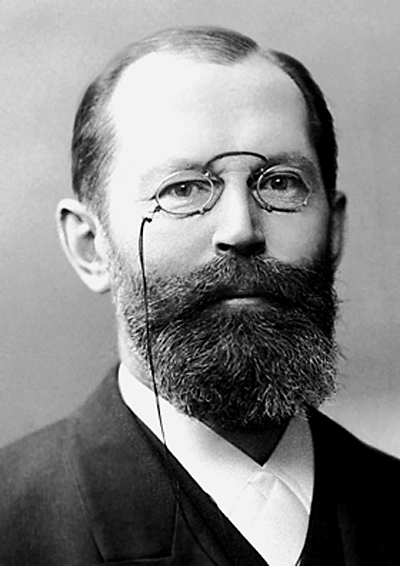
\includegraphics[width=\linewidth]{images/book3/fischer.jpg}
\end{minipage}\hfill
\begin{minipage}[t]{0.78\linewidth}
\vspace{0pt}
Emil Fischer établit, dès 1891, les configurations du glucose et de ses isomères, avant qu'aucune
méthode physique ne puisse voir une molécule~: en transformant les sucres les uns en les autres et en
comptant les stéréoisomères obtenus. La projection qu'il inventa pour les écrire porte encore son nom. Il
prépara aussi les premiers \omterm{def:b2:biomolecules:peptide}{peptides} de synthèse, et reçut le prix Nobel de chimie 1902. (Portrait~:
Atelier Victoria, Berlin, vers 1895, domaine public~; Wikimedia Commons.)
\end{minipage}
\end{history}

\section{Exercices}

\begin{exercise}[$\star$]\label{exo:b2:biomolecules:1}
Représenter l'alanine sous forme de \omterm{def:b2:biomolecules:amino-acid}{zwitterion}, puis les formes qui prédominent à pH 1 et à pH 12.
\end{exercise}

\begin{exercise}[$\star$]\label{exo:b2:biomolecules:2}
Calculer le \omterm{def:b2:biomolecules:amino-acid}{point isoélectrique} de la glycine, puis celui de l'alanine ($\mathrm pK_a$ 2.35 et 9.87).
\end{exercise}

\begin{exercise}[$\star$]\label{exo:b2:biomolecules:3}
Représenter le dipeptide Ala--Gly et entourer sa \omterm{def:b2:biomolecules:peptide}{liaison peptidique}. En quoi diffère-t-il de Gly--Ala~?
\end{exercise}

\begin{exercise}[$\star$]\label{exo:b2:biomolecules:4}
Dans une projection de Fischer avec \ce{COOH} en haut et la \omterm{def:b2:biomolecules:amino-acid}{chaîne latérale} \ce{CH2OH} en bas, le
\ce{NH2} de la sérine pointe vers la gauche. Est-elle D ou L~? Donner son descripteur CIP.
\end{exercise}

\begin{exercise}[$\star\star$]\label{exo:b2:biomolecules:5}
Donner la charge nette du tripeptide Lys--Gly--Asp à pH 1, 7 et 12.
\end{exercise}

\begin{exercise}[$\star\star$]\label{exo:b2:biomolecules:6}
Pourquoi utilise-t-on un \omterm{def:b2:biomolecules:peptide}{agent de couplage} pour former une \omterm{def:b2:biomolecules:peptide}{liaison peptidique}, plutôt qu'un \omterm{def:b2:acyl-substitution:derivative}{chlorure
d'acyle} de l'acide aminé protégé, préparé par le chlorure de thionyle et chauffé~?
\end{exercise}

\begin{exercise}[$\star\star$]\label{exo:b2:biomolecules:7}
Le D-fructose se cyclise par le \ce{OH} de C5 sur la cétone en C2. Donner la taille du cycle et
représenter le $\beta$-D-fructofuranose en \omterm{def:b2:biomolecules:anomer}{projection de Haworth}.
\end{exercise}

\begin{exercise}[$\star\star$]\label{exo:b2:biomolecules:8}
Les \omterm{def:b2:biomolecules:anomer}{anomères} purs du D-galactose ont des pouvoirs rotatoires spécifiques de $+150.7$ ($\alpha$) et de
$+52.8$ ($\beta$), et le mélange à l'équilibre $+80.2$ (données de l'exercice). Calculer la composition à l'équilibre.
\end{exercise}

\begin{exercise}[$\star\star$]\label{exo:b2:biomolecules:9}
Expliquer pourquoi le maltose réduit la liqueur de Fehling et pas le saccharose, et pourquoi le
saccharose la réduit après chauffage avec un acide dilué.
\end{exercise}

\begin{exercise}[$\star\star\star$]\label{exo:b2:biomolecules:10}
L'indice de \omterm{def:b2:acyl-substitution:saponification}{saponification} d'un corps gras est la masse d'hydroxyde de potassium, en mg, qui saponifie
1~g de ce corps gras. Le calculer pour la trioléine, \ce{C57H104O6}, et expliquer pourquoi un corps gras
à chaînes plus courtes a un indice plus élevé.
\end{exercise}

\begin{exercise}[$\star\star\star$]\label{exo:b2:biomolecules:11}
Planifier la synthèse de Gly--Ala à partir de la glycine et de l'alanine~: groupes protecteurs,
activation, couplage, déprotection, avec un couple orthogonal.
\end{exercise}

\begin{exercise}[$\star\star\star$]\label{exo:b2:biomolecules:12}
Écrire le brin complémentaire de 5$'$-ATGCGT-3$'$, à partir de son extrémité 5$'$, et compter les liaisons
hydrogène qui maintiennent le double brin.
\end{exercise}

\section{Problème~: l'aspartame}

\begin{problem}[{Problème du week-end --- les deux acides aminés et leurs configurations, la charge du
dipeptide en fonction du pH, sa synthèse et le problème $\alpha$/$\beta$, et son hydrolyse dans une
boisson gazeuse}]
\label{pb:b2:biomolecules:1}
L'aspartame est l'ester méthylique du dipeptide formé par le groupe carboxylique $\alpha$ de l'acide
L-aspartique et le groupe amino de la L-phénylalanine. Données~: $\mathrm pK_a$ de l'acide aspartique 2.0,
3.9 et 9.9 (valeurs modèles pour les groupes du dipeptide). Masses molaires (\unit{g/mol})~: C 12.011,
H 1.008, N 14.007, O 15.999.
% ledger: use:aspartame, pka:asp1, pka:asp2, pka:asp3, aw:C, aw:H, aw:N, aw:O

\medskip
\noindent\textbf{Partie I --- Les deux acides aminés.}
\begin{enumerate}
  \item Nommer les trois composés libérés par l'hydrolyse complète de l'aspartame.
  \item Représenter l'acide L-aspartique et la L-phénylalanine en projection de Fischer.
  \item Donner le descripteur CIP de chaque stéréocentre.
  \item Combien l'aspartame possède-t-il de stéréoisomères~?
  \item Représenter l'aspartame et repérer la \omterm{def:b2:biomolecules:peptide}{liaison peptidique} et l'ester.
  \item Pourquoi la configuration de chaque acide aminé importe-t-elle pour la saveur sucrée~?
\end{enumerate}

\medskip
\noindent\textbf{Partie II --- Charge en fonction du pH.}
\begin{enumerate}[resume]
  \item Énumérer les groupes ionisables de l'aspartame. Pourquoi l'extrémité C-terminale n'en fait-elle pas partie~?
  \item Avec les valeurs modèles, donner la charge nette à pH 2.
  \item Même question à pH 7.
  \item Même question à pH 12.
  \item Estimer le \omterm{def:b2:biomolecules:amino-acid}{point isoélectrique} dans ce modèle.
  \item Pourquoi les vraies valeurs de $\mathrm pK_a$ du dipeptide différeraient-elles de celles de l'acide
        aspartique libre~?
\end{enumerate}

\medskip
\noindent\textbf{Partie III --- Synthèse.}
\begin{enumerate}[resume]
  \item Pourquoi ne peut-on pas simplement chauffer ensemble l'acide aspartique et l'ester méthylique de la phénylalanine~?
  \item Quels groupes de l'acide aspartique faut-il protéger~?
  \item Quel est l'effet d'un \omterm{def:b2:biomolecules:peptide}{agent de couplage} sur le groupe carboxylique libre~?
  \item L'acide aspartique possède deux groupes carboxyliques. Que forme-t-on si l'on couple le mauvais~?
  \item Proposer une protection orthogonale qui ne laisse libre que le groupe carboxylique $\alpha$, ainsi que
        son retrait.
  \item Pourquoi ne faut-il pas laisser trop longtemps l'acide aminé activé en milieu basique~?
  \item Écrire la séquence des étapes.
\end{enumerate}

\medskip
\noindent\textbf{Partie IV --- Hydrolyse dans une boisson gazeuse.}
\begin{enumerate}[resume]
  \item Quelles liaisons de l'aspartame peuvent être hydrolysées dans une boisson acide~? Laquelle cède la première~?
  \item Donner les produits de l'hydrolyse de l'ester seul.
  \item Pourquoi une boisson ancienne a-t-elle un goût moins sucré~?
  \item Calculer la masse molaire de l'aspartame, \ce{C14H18N2O5}.
  \item Calculer la quantité d'aspartame dans une canette qui en contient \qty{180}{mg}.
  \item Donner la masse de méthanol libérée par l'hydrolyse complète de \qty{180}{mg}
        d'aspartame.
\end{enumerate}
\end{problem}
